\documentclass[a4paper,12pt]{scrartcl}
\usepackage[english]{babel}
\usepackage[utf8]{inputenc}

\usepackage{amsmath}
\usepackage{amssymb}

% CONTENTS
% 1. Introduction
% 2. Theory
% 3. User Manual for the Python Module

% * wir schauen den graphen fuer pi/3, pi/4, ... an und fuer diese scheint die Funktion zu konvegieren 

% Conclusion
% Bibliography

\title{Study of the Machine Precision via the Approximation of a Derivative}
\author{Christian Parpart, Kei Thoma}
\date{\today}

\begin{document}

\maketitle
\tableofcontents

\section{Theory}

Before we continue with our endeavour, it is a good idea to reiterate fundamental results of linear algebra.

\subsection{LU Decomposition}
\section{The Sweet Spot of the Increment}
To test our theory, we consider the following function
\begin{align*}
    g_1(x) := \frac{\sin{x}}{x} \text{,}
\end{align*}
and its derivatives
\begin{align*}
    {g'}_{1}(x) = \frac{x \cdot \cos{x} - \sin{x}}{x^2} \hspace{1cm} {g''}_{1}(x) = \frac{(x^2 - 2) \sin{x} + 2 x \cos{x}}{x^3} \text{}
\end{align*}
on the interval \(I := [\pi, 3\pi]\). Note that we are bounded by the limitation of a computer, i.e. the interval \(I\) is partitioned into \(p := 1000\) many grid points and only on these points the functions will be evaluated.


\subsection{Approaching the Approximation} % dont like the tile

We first want to get a picture of what we are working with. Therefore, using the Python module, we have drawn the plot of \(f\), its first two exact derivatives, \(D^{(1)}_h(x)\) and \(D^{(2)}_h(x)\). For the increment \(h\) we have chosen the following values
\begin{align*}
    \frac{\pi}{3} \text{,} \hspace{0.5cm} \frac{\pi}{4} \text{,} \hspace{0.5cm} \frac{\pi}{5} \text{,} \hspace{0.5cm} \frac{\pi}{10} \text{.}
\end{align*}
See figure \ref{fig:exp1_h} for the resulting graph.
\pagebreak

%%% figure the 4 plots for the h
\begin{figure}[h!]
    \centering
    \begin{subfigure}[b]{0.4\linewidth}
        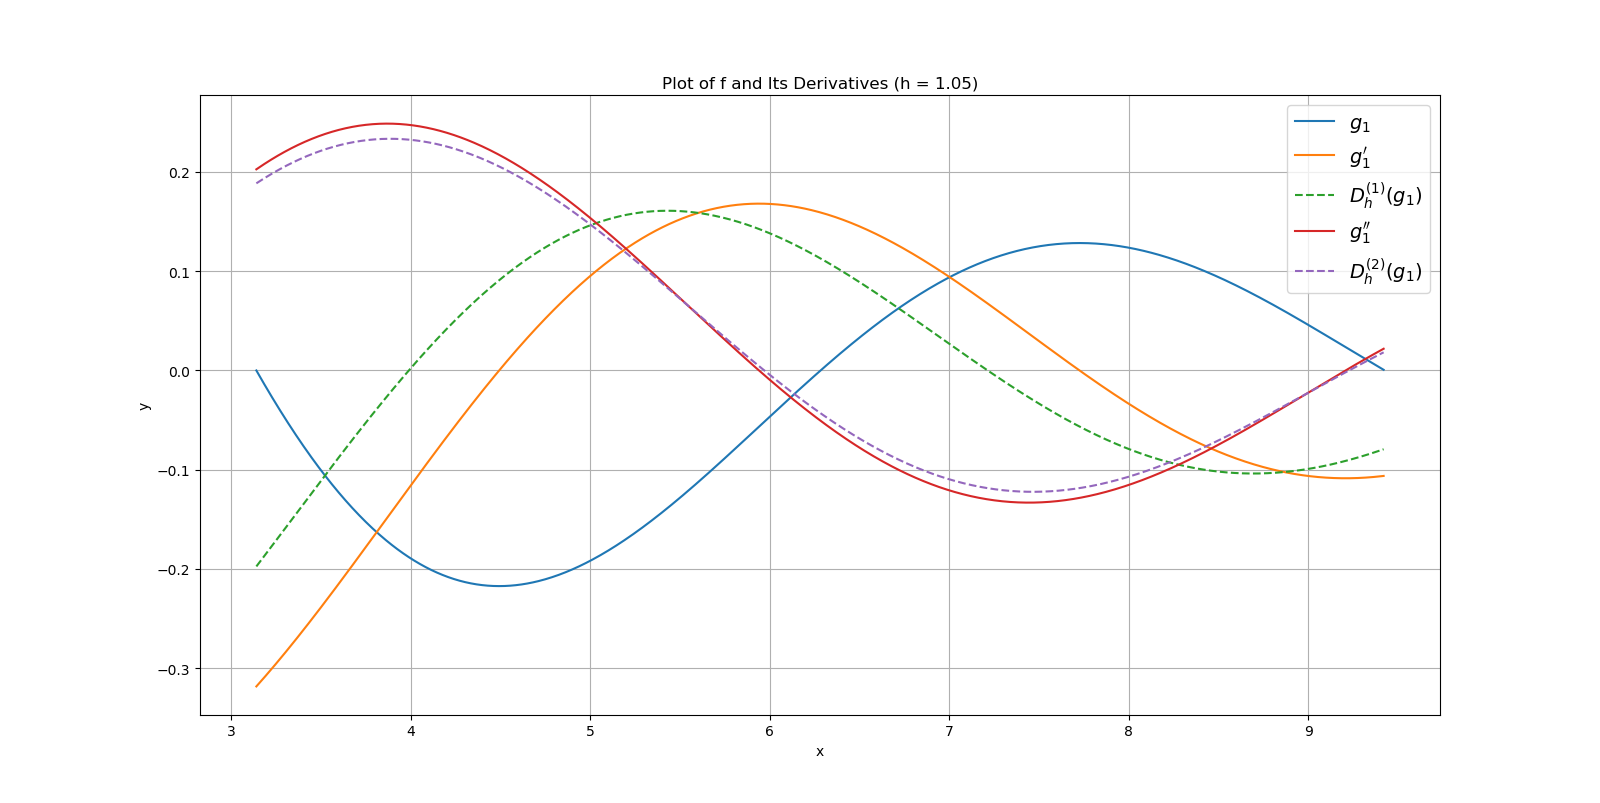
\includegraphics[width=\linewidth]{graphics/plot_h/exp1_huge_h.png}
    \end{subfigure}
    \begin{subfigure}[b]{0.4\linewidth}
        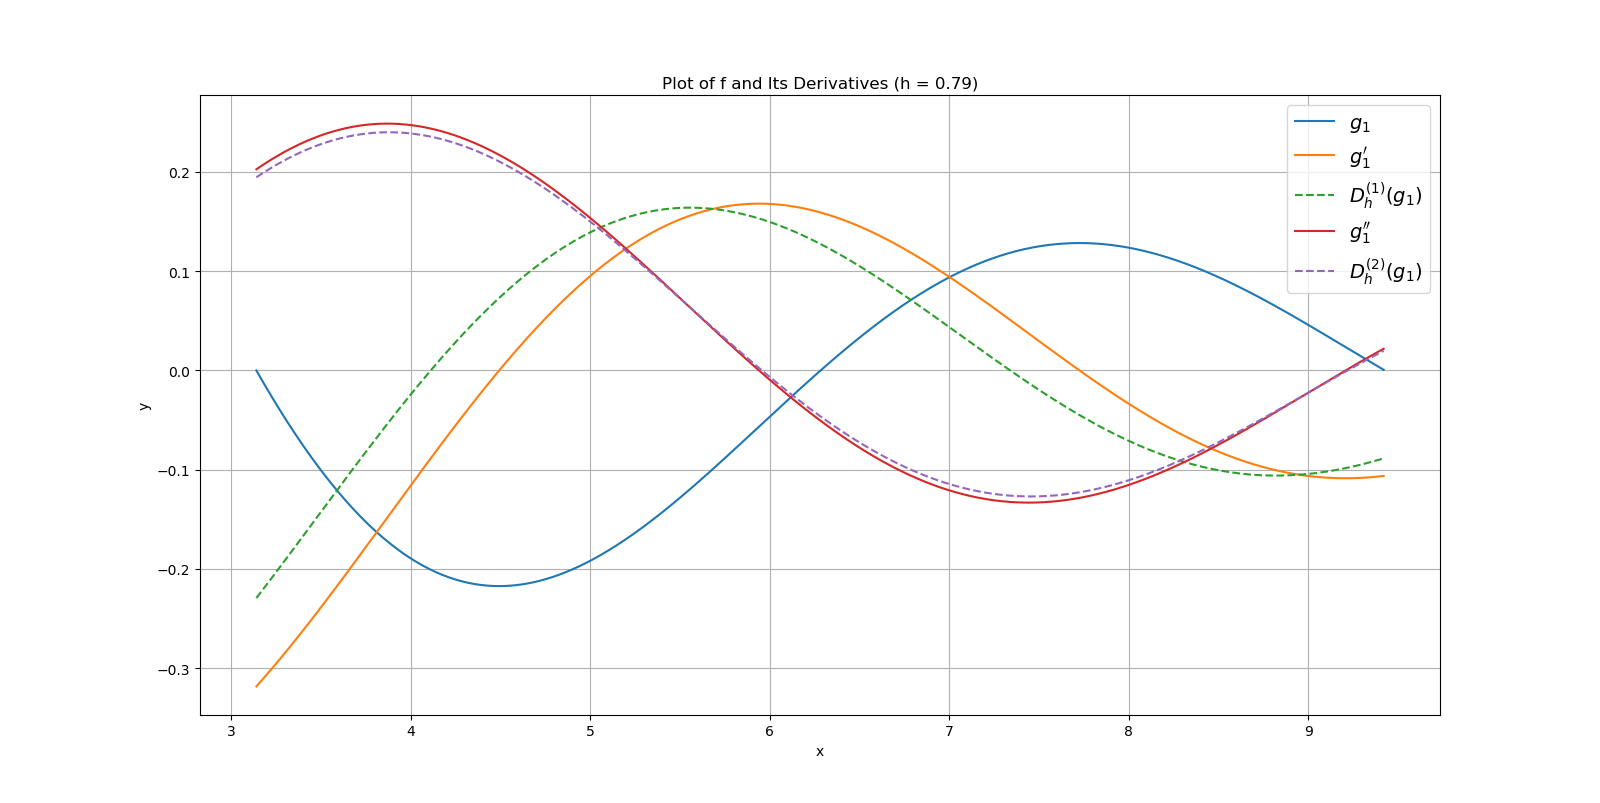
\includegraphics[width=\linewidth]{graphics/plot_h/exp1_large_h.png}
    \end{subfigure}
    \begin{subfigure}[b]{0.4\linewidth}
        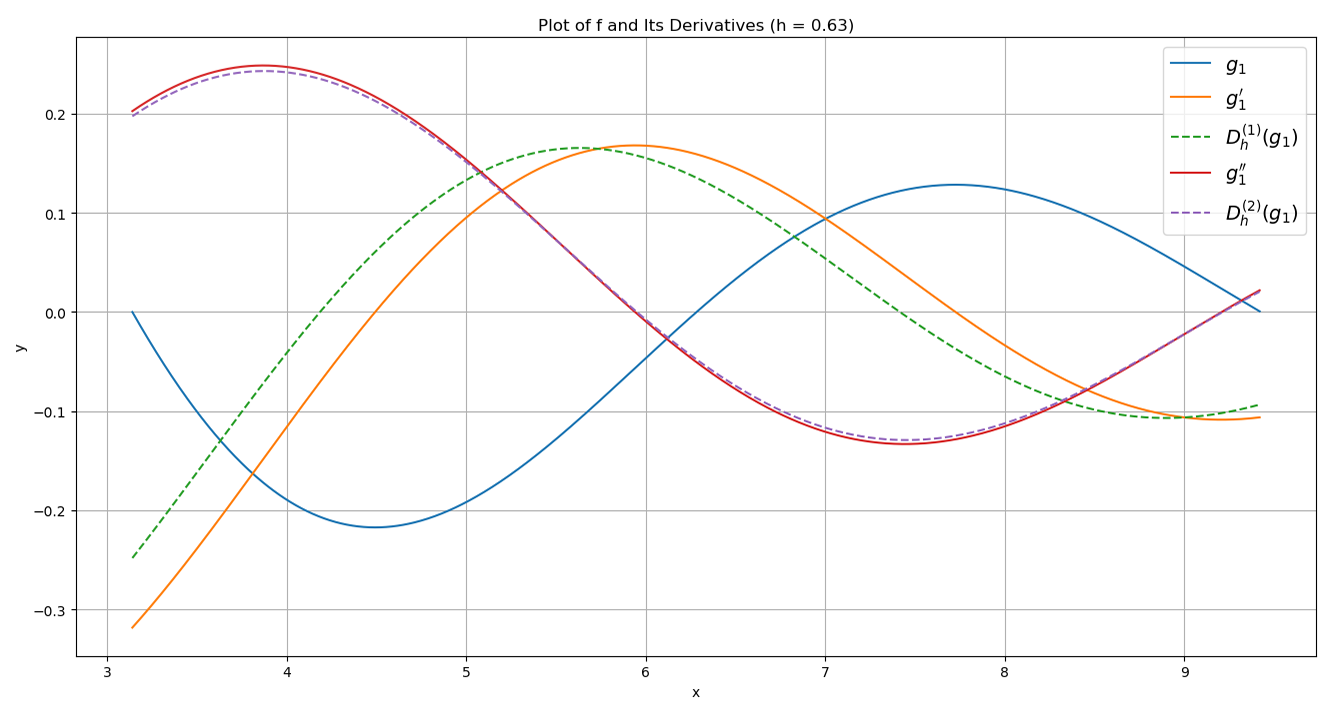
\includegraphics[width=\linewidth]{graphics/plot_h/exp1_small_h.png}
    \end{subfigure}
    \begin{subfigure}[b]{0.4\linewidth}
        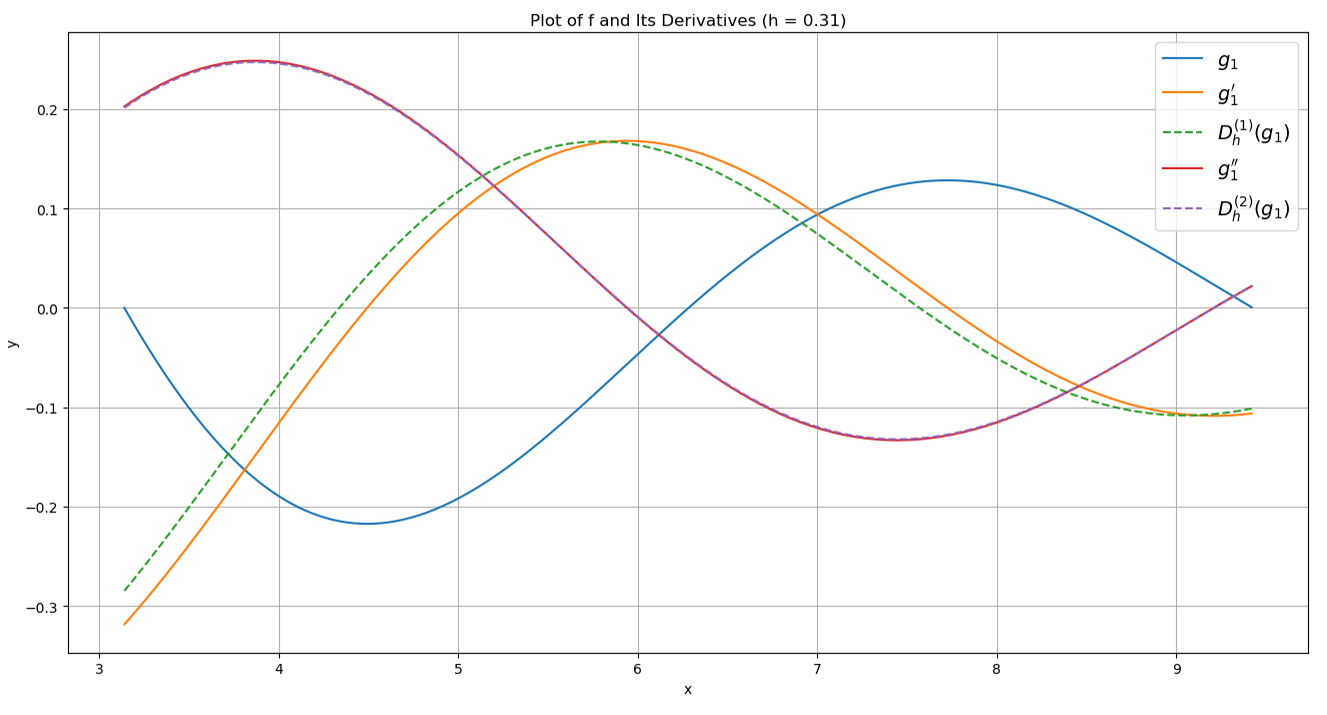
\includegraphics[width=\linewidth]{graphics/plot_h/exp1_tiny_h.png}
    \end{subfigure}
    \caption{huge}
    \label{fig:exp1_h}
\end{figure}

As one can clearly see, both \(D^{(1)}_h(x)\) and \(D^{(2)}_h(x)\) merges to the analytic derivatives of \(f\) as \(h\) becomes smaller. \(D^{(2)}_h(x)\) is almost indistinguishable from \(f''\) for \(h = \frac{\pi}{10}\). This result confirms the first part of the theory -- the approximation becomes better as the increment tends to \(0\). That \(D^{(2)}_h(x)\) converges faster to \(f''\) is also expected from the theory. But admittingly, even \(h = \frac{\pi}{10}\) is rather large if one compares it to the 64-bit precision we have worked with and most modern computers have to offer. Can we indefinitely improve our approximation if we just choose \(h\) to be small enough? Unfortunately, it turns out that this is not the case.

\subsection{The Anatomy of Errors}

Now, we consider the two errors \(e_f^{(1)}(h)\) and \(e_f^{(2)}(h)\) which are again, the largest disparity between the analytic and the approximation on the interval \(I\). We have drawn the plot (see \ref{xxx}) in double log scale for the error for
\[h \in [10^{-9}, 10^2] \text{.} \]

%%% figure of the error plot

Before we discuss the bad news, let us examine where the theory was right in its prediction. The middle part of \(e_f^{(1)}(h)\) and \(e_f^{(2)}(h)\) are parallel to the lines of \(h\) and \(h^2\) respectively. This is as we hypothesized since the order of convergence of the error are
\[\mathcal{O}(h) \hspace{0.3cm} \text{for} \hspace{0.3cm} e_f^{(1)}(h) \hspace{0.3cm} \text{and} \hspace{0.3cm} \mathcal{O}(h^2) \hspace{0.3cm} \text{for} \hspace{0.3cm} e_f^{(2)}(h) \text{.}\]
The left side of the plot, however, does not behave the way we wanted. At around \(10^{-8}\) for \(e_f^{(1)}(h)\) and at \(10^{-4}\) for \(e_f^{(2)}(h)\) both plots stop converging and starts increasing again. This means that on the machine number line the approximation does not uniformly converge to the analytic derivative. Instead, there is an optimal point for the increment, a "sweet spot", so to speak. Beyond this sweet spot, the approximation actually becomes worse and thus, we cannot decrease the value of the increment haphazardly in hopes of getting a better approximation.

But why does this happen? Where exactly in our computation does the imperfectness of the machine sneak in? To answer this question, see figure \ref{xxx}

%%% figure

Here, we have fixed \(x = \pi + 2 \approx 5.14\) to observe the behavior of the analytic derivatives and the approximations with \(h\) as the variable. At around \(10^{-8}\) and \(10^{-4}\) respectively, both \(D^{(1)}_h(x)\) and \(D^{(2)}_h(x)\) starts oscillating even though in theory, these blue curves should once again smoothly approach the exact solution of \(f'\) and \(f''\) at \(x = \pi + 2\). This oscillation results in the error not converging.

Therefore, we proceed by looking at the definition of the approximation. We had
\begin{align*}
    D^{(1)}_h(x) &:= \frac{f(x + h) - f(x)}{h} \\
    D^{(2)}_h(x) &:= \frac{f(x + h) + f(x - h)- 2 f(x)}{h^2} \text{.}
\end{align*}
% here maybe we could takl about the conditioning of f?
For \(D^{(1)}_h\), if \(h\) becomes small enough, then \(g_1(x + h) \approx g_1(x)\) since \(g_1\) is continuous. Hence at the numerator, we are essentially subtracting two numbers which are close to each other, but such subtractions are ill-conditioned (see \cite{Lecture}). In other words, for \(h\) which are small enough, we loose accuracy at this point of the approximation process resulting in the error graph we have seen at \ref{XXX}. Similar argumentation also works for the second derivative as \(f(x + h) + f(x - h) \approx 2 f(x)\) for small \(h\).

It is important to keep in mind that the threshhold for \(h\) being \textit{small enough} depends on the machine precision used for the computation. Our result is based on a 64-Bit float and while in general, the approximation will never converge to the analytic derivative outside of our mathematical imagination, the exact spot where the error stops decreasing might differ.
\section{j-Variable Variations}

In the preceding section, we have learned that the computer is indeed limited and for every type of float there is an optimal increment for an approximation. To advance our understanding in this particular subject, let us modify the function and observe the effect on the error. Define
\begin{align*}
    g_j(x) := \frac{\sin(j x)}{x} \text{,}
\end{align*}
and we have the derivatives
\begin{align*}
    g_j'(x) &= \frac{j x \cos(jx) - \sin(jx)}{x^2} \\
    g_j''(x) &= \frac{(2 - j^2 x^2)\sin(jx) - 2 j x \cos(jx)}{x^3} \text{,}
\end{align*}
with \(j > 0\). Once again, we will evaluate these functions on the partitioned interval \(I = [\pi, 3\pi]\) with \(p = 1000\). But given \(g_j\), how does large and small \(j\) affect the error plot?

%%%
\begin{figure}[h!]
    \centering
    \begin{subfigure}[b]{0.49\linewidth}
        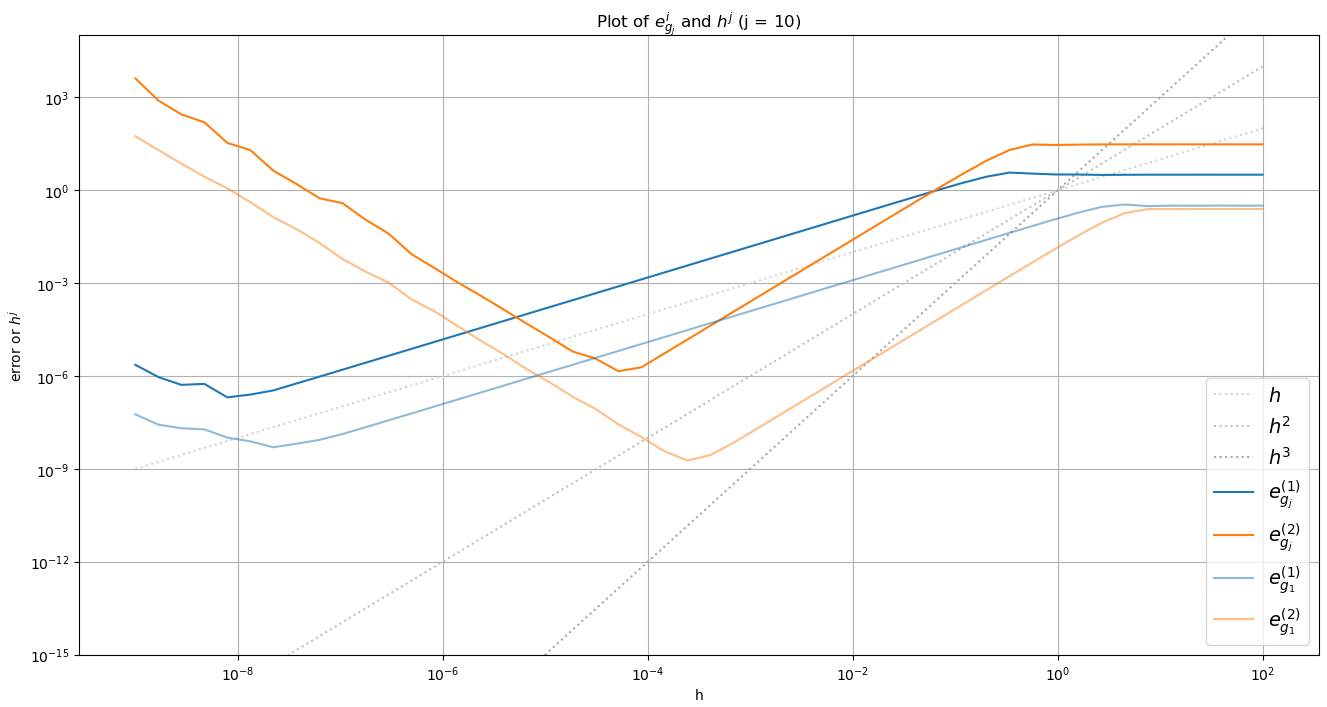
\includegraphics[width=\linewidth]{graphics/j_error_plot/big_j.png}
    \end{subfigure}
    \begin{subfigure}[b]{0.49\linewidth}
        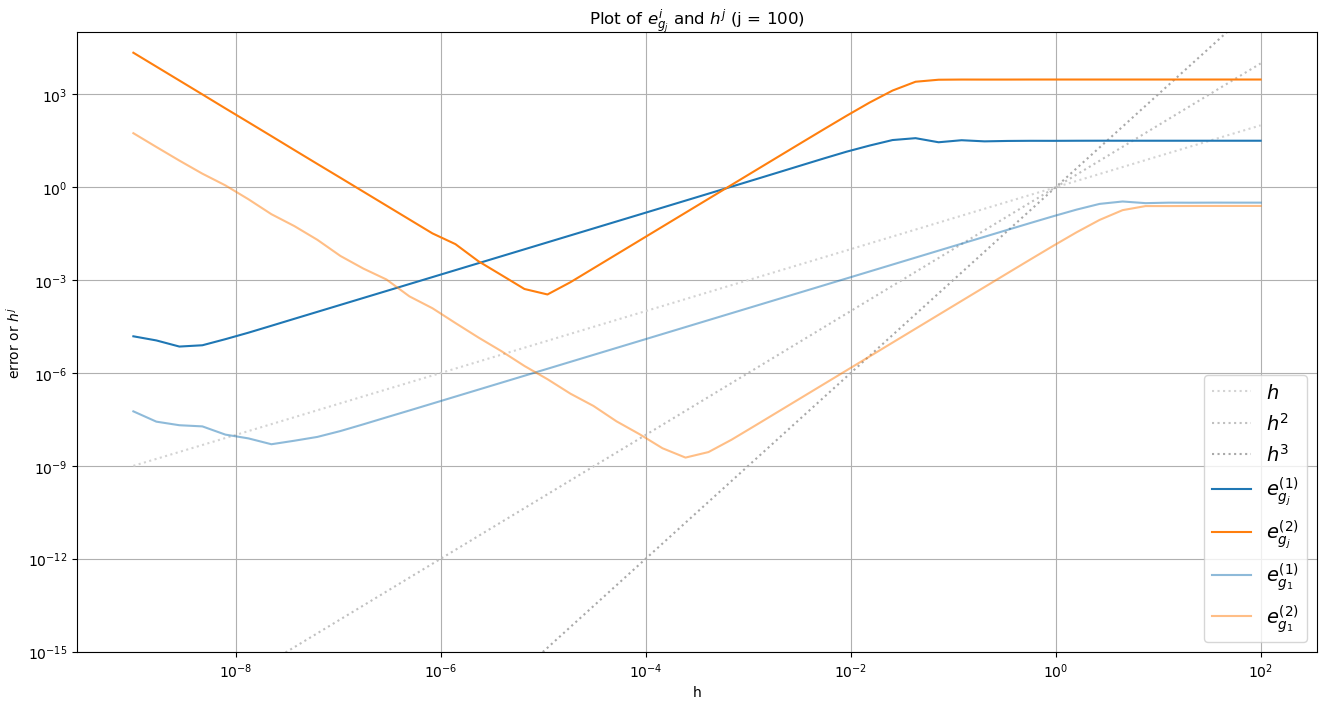
\includegraphics[width=\linewidth]{graphics/j_error_plot/large_j.png}
    \end{subfigure}
    \begin{subfigure}[b]{0.49\linewidth}
        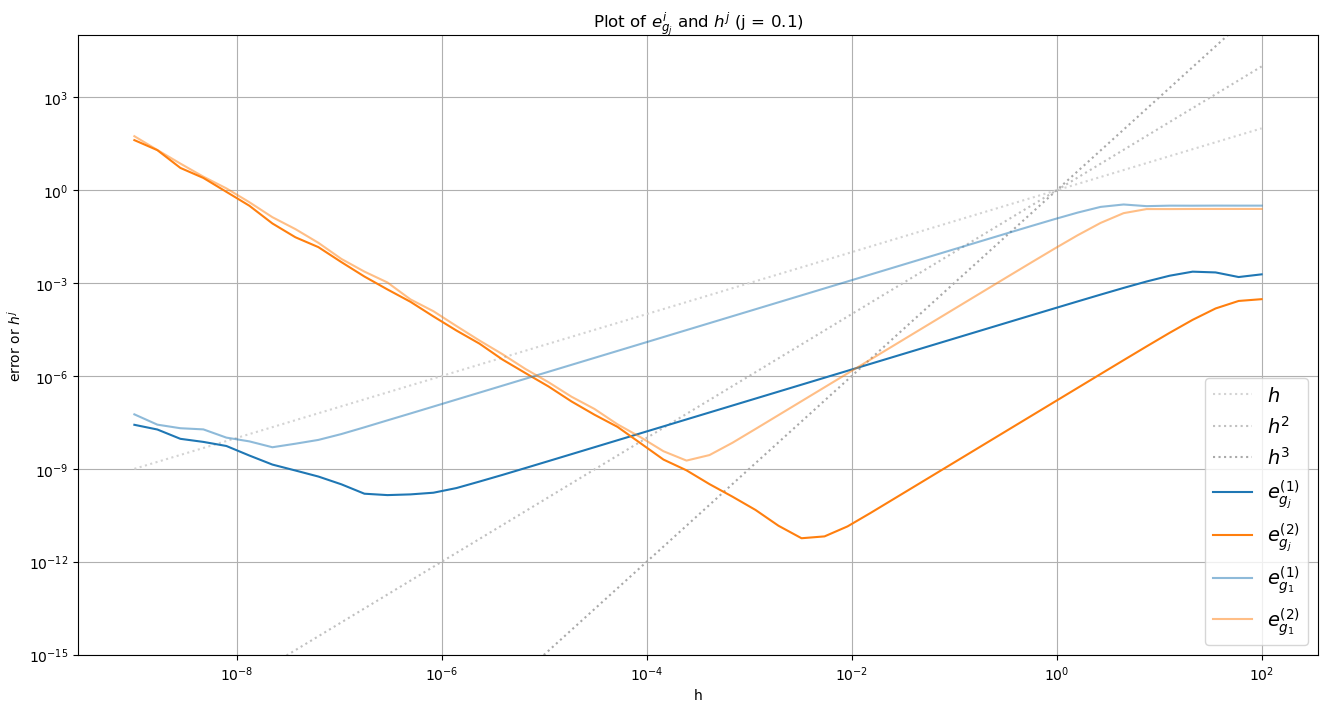
\includegraphics[width=\linewidth]{graphics/j_error_plot/small_j.png}
    \end{subfigure}
    \begin{subfigure}[b]{0.49\linewidth}
        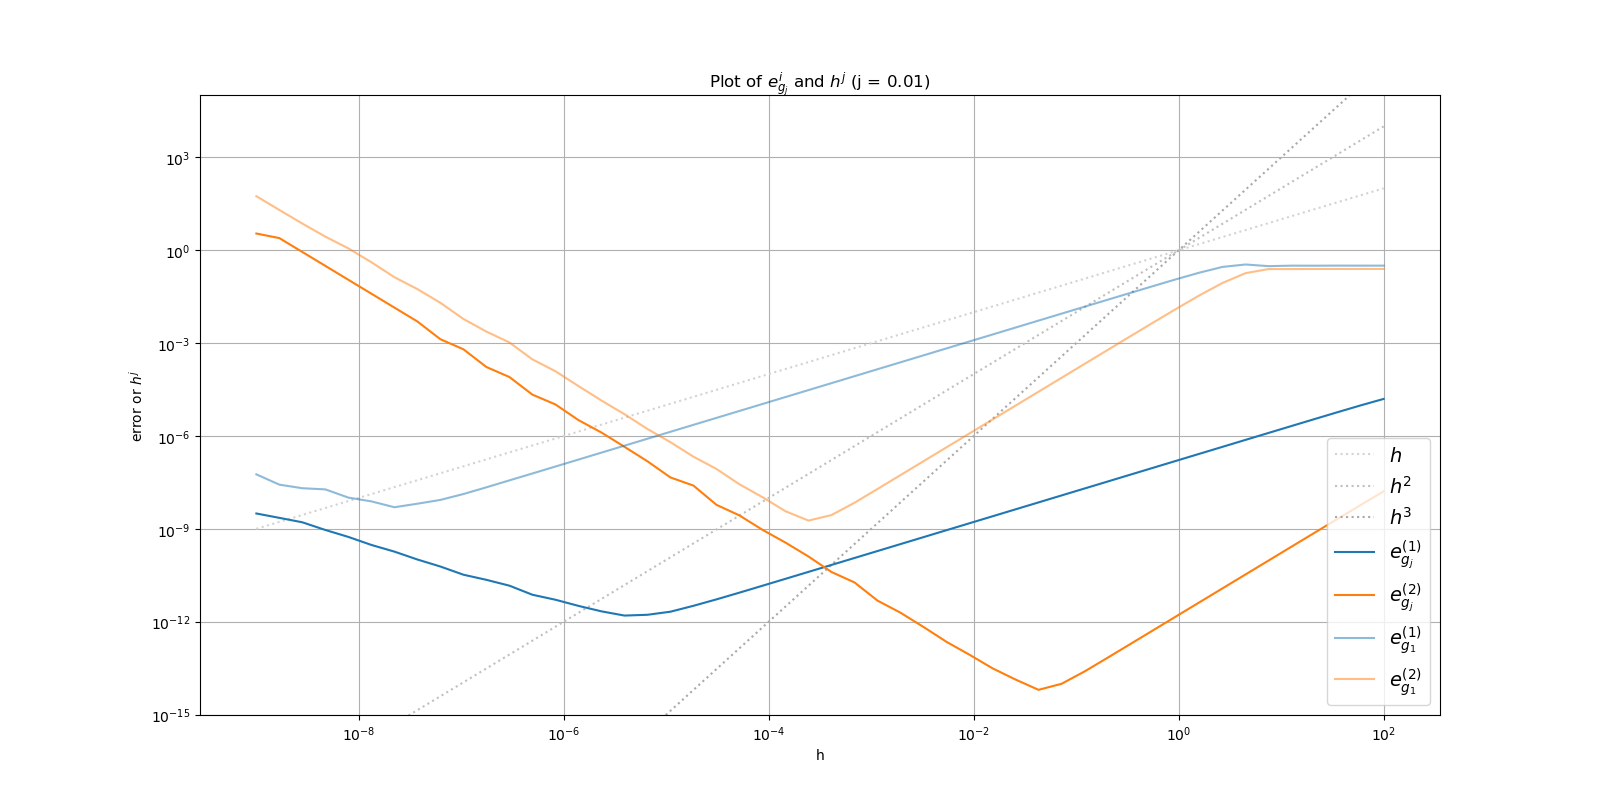
\includegraphics[width=\linewidth]{graphics/j_error_plot/tiny_j.png}
    \end{subfigure}
    \caption{j-variable variations}
    \label{fig:exp2_j}
\end{figure}

On the figure \ref{fig:exp2_j} one can see that as \(j\) gets smaller, the sweet spot of the increment for both \(D^{(1)}_h(g_j)\) and \(D^{(2)}_h(g_j)\) moves to bottom right. This means, that the optimal choice for \(h\) becomes larger and the approximation becomes slightly better. On the other hand, choosing big values for \(j\) moves the spot to the top left which means that one needs a smaller \(h\) for the most optimal yet worse approximation.
Why does this movement of the sweet spot occur? To answer this question, we have to look at what \(j\) does in our function \(\sin(\cdot)\). \(j\) changes the period, the smaller the \(j\) the smaller the period and vice versa. Because \(g_j\) is once again a periodic function\footnote{A function \(f\) is periodic if there is a nonzero constant \(P \in \mathbb{R}\), such that \(f(x + P) = f(x)\) for all \(x\) in the domain.}, this property of periodicity is inherited from \(\sin(\cdot)\). If we now consider once again how the approximation is calculated, we had

\begin{align*}
    D^{(1)}_h (g_j) = \frac{g_j(x + h) - g_j(x)}{h} \text{.}
\end{align*}

We know that the subtraction at the numerator is the source inaccuracy. If \(j\) is small however, then \(g_j(x + h) - g_j(x)\) because the small change in the variable results in small change in value. Therefore, the approximation approaches the exact one with a larger increment. Hence the optimal increment is larger and gives a better approximation (in the sense that the error is small). Similary, if \(j\) is large, then for a better approximation one needs a smaller \(h\).
\section{User Manual}

First of all, since the successive over-relaxation is an iterative algorithm, we need a termination condition. In this protocol, we will use the following conditions, \(\epsilon = \frac{1}{10^{-8}}\) is the tolerance for the norm of the residual in the infinity norm, \(\texttt{max\_iter} = 1000\) is the number of maximum iteration, and \(\texttt{min\_red} = \frac{1}{10^{-4}}\) is the minimal reduction of the residual in the infinity norm in every step.

All results in this protocol can be found in the Python file \texttt{protocol.py}. Furthermore, one can change the global variable \texttt{PRESET} and \texttt{MAX\_N} at the top to alter the plots produced by the module. Alternatively, the function parameters can be edited in the main function.

\begin{thebibliography}{2}

\bibitem{H.Amann}
Herbert Amann, Joachim Escher
\textit{Analysis I} (German). 
3rd edition, Birkh{\"a}user Verlag, Berlin, 2006.

\bibitem{Lecture}
Caren Tischendorf
\textit{Numerische Lineare Algebra} (German).
Lecture at Humboldt University of Berlin, Winter Semester 2019/20.

\end{thebibliography}

\end{document}